%*******************************************************************************
%*********************************** First Chapter *****************************
%*******************************************************************************

\chapter{Virtual reality – theoretical background}\label{chapter1}  %Title of the First Chapter

\epigraphhead[40]{\epigraph{\textit{Reality is merely an illusion, albeit \linebreak a very persistent one.}}{{Albert Einstein}}}

\ifpdf
    \graphicspath{{Chapter1/Figs/Raster/}{Chapter1/Figs/PDF/}{Chapter1/Figs/}}
\else
    \graphicspath{{Chapter1/Figs/Vector/}{Chapter1/Figs/}}
\fi


%********************************** %First Section  **************************************
\section{Definition} %Section - 1.1 

	Nowadays, thanks to constant technology development, accessibility of Internet and computer-related innovations, people
tend to live parallelly in two worlds- real and virtual. As the latter one offers less boundaries and constraints, and the only limit there is, is people's imagination, it is not surprising that these days one can observe growing trend in improving the quality of man's immersion in artificial world. This possibility leads to the new idea of perceiving the surrounding reality, which is called Virtual Reality (VR) or Virtual Environment (VE).

	The concept of VR has never been unified, therefore it cannot be defined in one way. One of the most general definition explains it as "an immersive and interactive system that provides users with the illusion of entering a virtual world" \cite{Heim98}. In other papers one can find more specific description. Most of them state that three- dimensional graphics is an essential part of VR \cite{Fuchs92}, moreover, that it needs to provide a multi-sensory computer-mediated environment \cite{Cruz93}. Despite the multitude of possible definitions, all of them agree that VE is immersive, interactive and that it creates an experience in simulated world. It is well systematized by Sherman and Craig \cite{Sherman03}, who describe four essential elements in VR, which are:
\begin{itemize}
\item \textbf{Virtual world}– set of objects in a space, relationship between them and laws that govern this entirety.
\item \textbf{Immersion}– impression of being present in showed environment instead of looking at it from the outside. This phenomenon will be described more precisely in section \ref{imm}.
\item \textbf{Sensory feedback}– collection of sensory data about the environment based on user input, for example his position which determines the given view and perspective.
\item \textbf{Interactivity}– responsiveness to user actions.
\end{itemize}
Those features of Virtual Reality draw it away from traditional media technologies and thus VE gives new possibilities which has never been considered before.
	
	In this section it is worth mentioning other notions, closely related to VR, which are Real Enovironment (RE), Mixed Reality (MR) Augmented Reality (AR) and Augmented Virtuality (AV). For this purpose it is convenient to introduce the concept of Reality-Virtuality Continuum, which is presented below, in Figure \ref{fig:continuum}.
\begin{figure}[h] 
\centering    
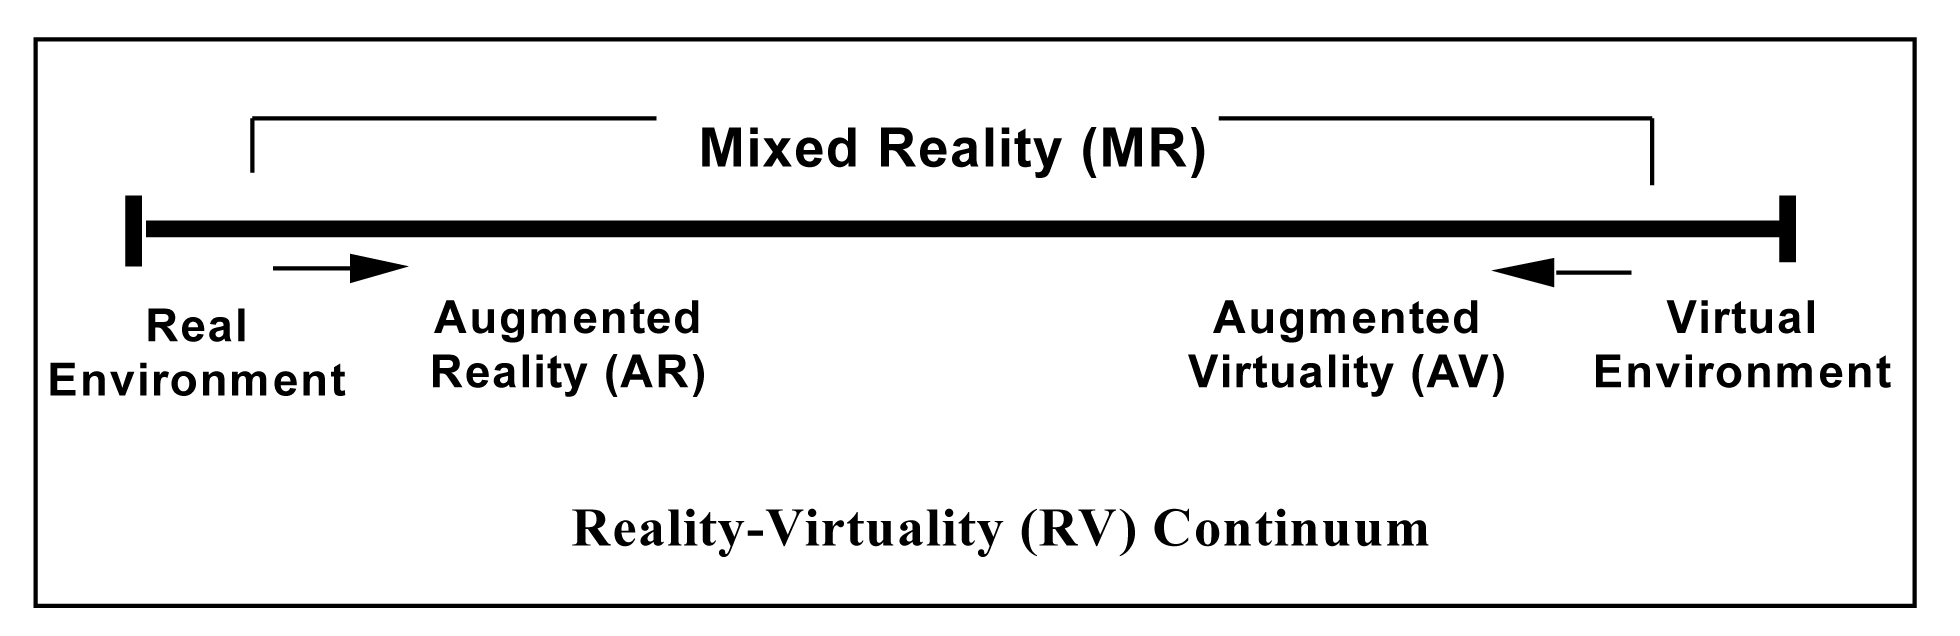
\includegraphics[width=1.0\textwidth]{Figs/rv_continuum.jpg}
\caption{Representation of Reality-Virtuality Continuum \cite{Milgram94}.}
\label{fig:continuum}
\end{figure}
\\As shown, the Real Environment is an opposite idea to the one that was already explained, which is Virtual Reality. Thus one can understand it as an environment, which consists of the real objects exclusively, observed either in person or through some kind of display or window. Between those two extrema of RV, the Mixed Reality is placed. It is a general notion, which describes surrounding, where both real and virtual objects are presented together. While going into details, two subconcepts occur. First one, Augmented Reality, may be defined as "augmenting natural feedback to the operator with simulated cues" \cite{Milgram94}, what practically means that the user display is transparent, so it shows the view of a real world, but additionally enriched with coexisting virtual objects. Ipso facto, Augmented Virtuality is very close to AR, as the only difference between them is stated by proportions of virtuality and reality presented to the user, what results from Figure \ref{fig:continuum}. It follows, therefore, that those two concepts interpenetrate.


	 
%********************************** %Second Section  *************************************
\section{History}\label{history} %Section - 1.2 

It may seem that Virtual Reality is an idea that originated with a recent rapid technological development. In fact, VR's origins date back to 1950s at the latest, when the first devices for that purpose were designed.

In 1957 the machine called \textit{Sensorama} (Figure \ref{fig:sensorama})  was constructed by Morton Heiling. This multi-sensory stimulator contained prerecorded film in color and stereo (six to choose), binaural sound and, additionally, scent, wind and vibration effects. Although it was not interactive, \textit{Sensorama} is considered as the first Virtual Environment system.
\begin{figure}[h] 
\centering    
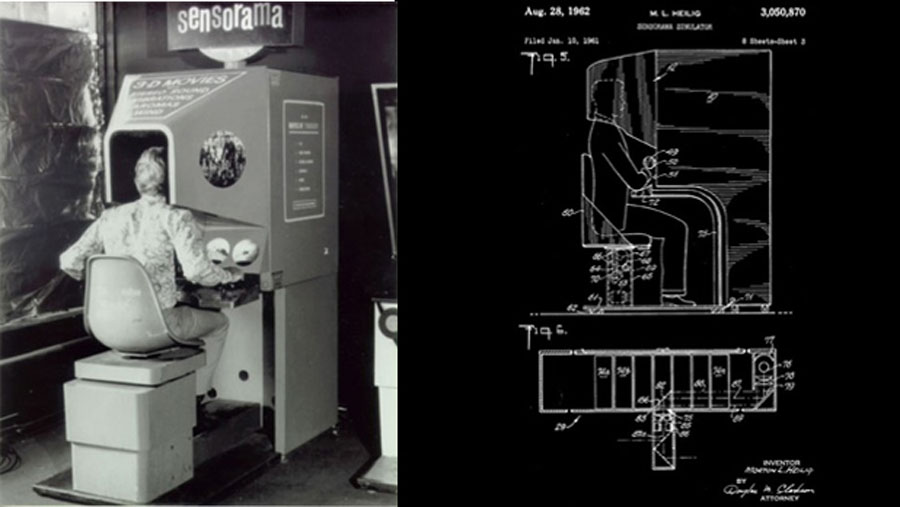
\includegraphics[width=0.8\textwidth]{Figs/sensorama.jpg}
\caption{\textit{Sensorama}, patented in 1962 \cite{Olszewski15}.}
\label{fig:sensorama}
\end{figure}
Four years later, Philico Corporation produced another device- the \textit{Headsight}, which was the first example of Head-Mounted Display (HMD) with motion tracking. It provided a vision of a film that was recorded in a real time by cameras, what makes it an Agumented Reality rather than VR system.
Subsequently, in 1965, Ivan Sutherland, proposed the concept of \textit{The Ultimate Display}. The assumptions he declared, encompass the Virtual Reality idea until today. These were virtual world maintained in real time through a computer hardware, user's ability to interact with it and a tactile feedback, all with usage of HMD and augmented 3D sound. On this basis he created      
\textit{The Sword of Damocles}, device with Head-Mounted Display and head-tracking. Although its large size and weight, it was invested in by NASA and CIA \cite{Olszewski15, Mandal13}.

1970s brought another new, innovative ideas, like \textit{GROPE}- prototype of a force-feedback system or \textit{VIDEOPLACE}- artificial reality, where position-tracked silhouette of a user was projected on a screen as an avatar. But the most rapid development occured in the next decades, when the miniaturisation went hand in hand with expenses reduction. In 1985 and 1988, the VPL company introduced first commercially available VE devices- \textit{DataGlove} and \textit{EyePhone} HMD. Next, in 1989, Fake Space Labs manufactured \textit{BOOM}, which was a small box with two CRT monitors creating the stereoscopic view and a mechanical arm measuring the position of a box, what allows the user move through a virtual world. Another concept, that did not base on Head-Mounted Display, was presented three years later as the \textit{CAVE}- Cave Automatic Virtual Environment. Here, the stereoscopic images were projected on the walls of a room and could be interpreted properly thanks to LCD shutter glasses worn by a user. Comparing to HMD solutions, \textit{CAVE} assured wider field of view and better quality of presented images. In the decade of 1990s the strongest interest was shown in games industry as a VR's application. This resulted into several systems, like \textit{Virtuality}, \textit{Sega VR} or \textit{Virtual Boy}, which often showed poor image quality or even caused adverse health effects (nausea or headache) to the user \cite{Olszewski15, Mandal13}. 

After the strong 3D graphics development, in 2012, young constructor Palmer Luckey created a new HMD-based device called \textit{Oculus Rift}, that met with a great commercial interest. Two years later, Oculus VR company was bought for a 2,5 billion of dollars, what accelerated a present growth of Virtual Reality development \cite{Olszewski15}. Current used software and hardware are described in section \ref{har} and \ref{dev}.
 
%********************************** %Third Section  *************************************
\section{Hardware and software}\label{har}%Section - 1.3

First of all, to understand how does the Virtual Reality really works, one has to become familiar with the basic components of those systems and their architecture. Generally, in VE systems, user is connected as part of the input/output loop, providing input through devices for interaction and experiencing the result of this input through variety of output, immersive devices. VR engine (computer) is responsible for processing loop information in real-time. Figure \ref{fig:architecture} presents the scheme of those dependencies.
\begin{figure}[h]
\centering    
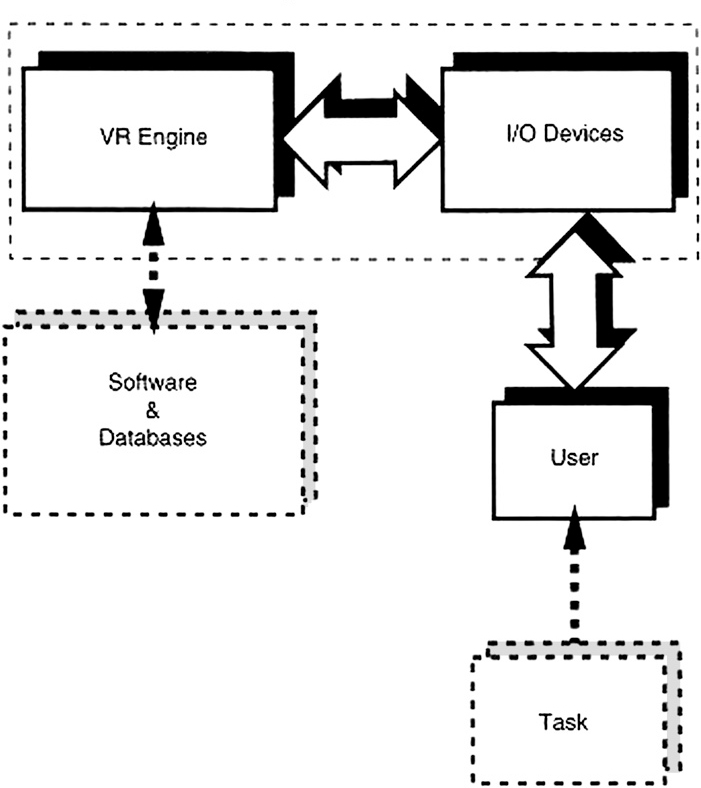
\includegraphics[width=0.5\textwidth]{Figs/architecture.jpg}
\caption{Architecture of Virtual Reality system. I/O stands for input/output \cite{Lange10}.}
\label{fig:architecture} 
\end{figure}
\subsection{Immersion}\label{imm}%Subsection - 1.3.1
Sensation of immersion can differ qualitatively, therefore, on this basis, Virtual Reality is divided into three groups \cite{Mandal13}:

\begin{enumerate}
\item Non-immersive systems
\item Semi-immersive systems
\item Immersive systems
\end{enumerate}

The first one which is called, interchangeably, Desktop-VR systems or WOW (Window on World), is a simplest type of VE. It does not employ special devices, since it is based on working of one or more computer screens (mostly monoscopic). It allows interaction of user, but does not give him an impression of immersion and barely blocks out the real world. Therefore in some quarters it is not considered as Virtual Reality technology. Semi-immersive systems (Fish Tank VR) are improved versions of Desktop-VR, as they use not only screens, which are often stereoscopic in this case, but also head-tracking devices, that intensify immersion of a user. As they do not provide sensory feedback, they cannot be recognized as the third category of systems. Fully immersive systems, besides supporting stereoscopic vision, employ Head-Mounted Display which enables to, according to user input (position, orientation), change the view of the scene. Thanks to that, user may look and move around, so simply navigate in the virtual world which, additionally, is presented in full scale. Moreover, the immersion effect may be upgraded by sensory, auditory and haptic interfaces \cite{Mandal13, Brooks99}. 

Depending on the application and developer invention, user may achieve different types of immersion, which are listed below \cite{Mandal13}:
\begin{itemize}
\item Sensory immersion- feeling of entering into the virtual world and being stimulated intellectually by it. Experience of time and space unity because of the fusion with image medium.
\item Spatial immersion- occurs when the simulated world is perceptually convincing.
\item Narrative immersion- experience of being gripped in a story presented in virtual world.
\item Tactical immersion- occurs when user performs tactile actions that involve skill.
\item Strategic immersion- analytical involvement associated with mental challenge.
\item Psychological immersion- confusing the virtual surrounding with real life.
\end{itemize}
\subsection{Sensory feedback- output}%Subsection - 1.3.2
In simulating artificial world, the most important role plays stimulating user's senses. Thus, knowing the contribution of each one for information passed to humans brain, is very useful. Figure \ref{fig:senses} explains why the visual part of VR has become a focus of research and why the sense of sight appeals to people imagination the most. 
\begin{figure}[h]
\centering
\begin{tikzpicture}
\tikzstyle{every node}=[font=\scriptsize]
\pie [scale font, radius=3.5, rotate = 198, color ={black!10,black!20,black!30,black!40,black!45}] {70/Sight, 20/Hearing, 5/Smell, 4/Touch, 1/Taste}
\end{tikzpicture}
\caption{Five human senses contribution in information transfering to a brain \cite{Mazuryk96}.}
\label{fig:senses}
\end{figure}
Despite this fact, other senses are also taken into consideration of Virtual Environment systems research, what is presented below in this section. 
\subsubsection{Sight}\label{sight}
Human vision is stereoscopic, as each eye can see one two-dimensional image which partly overlap. Those images are being processed by a human brain obtaining a parallax effect- visual phenomenon of depth perception, based on a difference in position of each eye. This phenomena is mimicked by devices simulating three-dimensional vision, the most important ingredient in Virtual Reality- they generate different images for each eye performing natural dimensions and high resolution. 

The simplest gear to obtain stereoscopic vision are anaglyphic glasses. Each lens there has a different color, which acts as color filter, dividing an image in two sub-images. Another device is called shutter glasses, which have LCD screen in front of each eye. They are switched on interchangeably, corresponding with an image presented on a screen resulting in a 3D image \cite{Lacrama07}.
Next example, Fish Tank VR systems, use 3D glasses and standard desktop monitor. In this case, stereoscopic images are created with usage of the off-axis projection, the method that generates two asymmetrical (not centered on the main projection axis) projections.
\begin{figure}[h]
\centering    
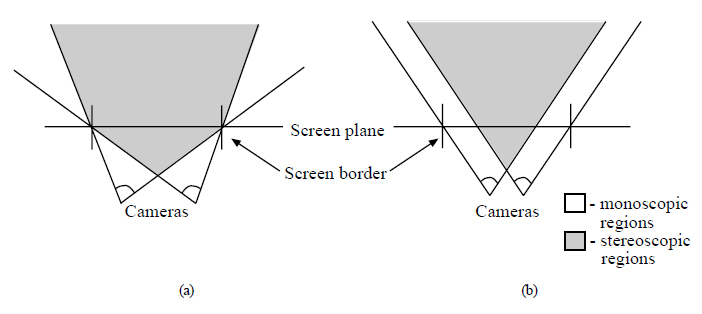
\includegraphics[width=0.9\textwidth]{Figs/projections.jpg}
\caption{Two centers of projection trasnformations: a) off-axis projection b) on-axis projection \cite{Mazuryk96}.}
\label{fig:projections} 
\end{figure} 
Nevertheless, in the subject of Virtual Reality, the most often used devices nowadays are immersive systems, like Head-Mounted Display, where different image displayed for each eye result in a stereoscopic effect. It may be obtained both by on-axis projection (when both image positions are on the symmetry axis of the view plane) or off-axis projection. The latter one is often needed since the tracked head position is not defined only by the axis of view plane. In modern systems the choice is up to the application developer \cite{Mazuryk96, Wikibook15}. The difference between those two approaches is shown in Figure \ref{fig:projections}.

Another issue discussing the vision is the field of view (FOV). Theoretically, human eye retains FOV of 180° both horizontal and vertical. Practically, this value is reduced to 150° because of the obscurement with cheeks, eyebrows and nose. Total horizontal viewing range binocularly overlaps in 120° (when focused on infinity). Since the task of Virtual Reality is to give sensations that are close to real ones, FOV is a parameter of high importance and it may be noticed in HMDs development. As example, current devices use the barrel distortion (Figure \ref{fig:tuscany})- technique that distorts image and enables lenses to present wider FOV, mimicking spherical shape of the eye \cite{Parisi15}.  Typical headset in 1996 supported 40°-60° field of view, while \textit{Oculus Rift} or \textit{HTC Vive} in 2015 covered 110°. For comparison with traditional visualisations, a 21" monitor observed from distance of 50 cm reaches 48° \cite{Mazuryk96, Oscillada15}.
\begin{figure}[h]
\centering    
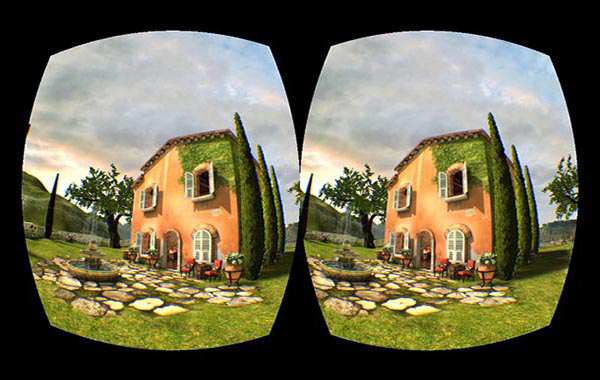
\includegraphics[width=1.0\textwidth]{Figs/tuscany.jpg}
\caption{VR Demo rednered in stereo with \textit{Oculus Rift} using barrel distortion \cite{Parisi15}.}
\label{fig:tuscany} 
\end{figure} 

\subsubsection{Hearing}
When vision does not provide enough information, auditory channel grows in importance. It may give an extra information (enabling perception of data outside the FOV) and may help in spatial orientation. Indeed, 3D sound in VR increases the level of immersion by simulating distances, directions and material information about the surrounding.

Spatial hearing in humans occurs by appraising both monaural (the same for both ears) and binaural (different for each eardrum) clues. The latter occur, if the sound source is placed outside the median plane- the distance between it and each ear is different, causing interaural differences of time (ITD) or intensity (IID). Those phenomenons are mainly used for directivity perception, which is an accurate tool (up to one degree), but only works in case of laterally localizing. On the other hand, monaural cues provide information about elevation: amplifications and attenuations in the frequency bands (intervals in frequency domain). These clues are needed in front/back localization. To recognize the direction in this case, humans rely on spectral modifications of sound caused by the shape and size of a head, neck, torso and outer ears. It is possible since the sound interacts with the body geometry differently, depending on its direction. All these subtle signals received by humans brain through the ears generate the effect of spatial sound perception \cite{Mazuryk96, Gobbetti99, Oculus16}. 

Thus to create a good immersion audio effect, one has to take into account not only the dependencies presented above, as they reffer to directional recognition only. Introducing sound changes while moving past listener (doppler shifts), considering environment geometry, distances (usually as a consequence of loudness) and material properties of objects (which may generate echoes) should also be done. Finally, sound and visual events need to be synchronized \cite{Mazuryk96, Gobbetti99}.
Therefore, to achieve successful acoustic simulation, three basic steps are required \cite{Mazuryk96}:
\begin{enumerate}
\item Sound generation- creating sounds, either by sampling or synthesizing, needed in the virtual world.
\item Spatial propagation- calculation of movement of sound waves through the environment.
\item Mapping of parameters- mapping calculated parameters from second step onto sounds that will be delivered through headphones or speakers to the user, with consideration of monaural and binaural clues to achieve the directional effect.
\end{enumerate}

According to the \textit{Oculus Rift} documentation, to accomplish second and third step in \textit{Oculus} device, the Head-Related Transfer Functions (HRTF) referring to directional recognition are applied. HRTF data may be obtained both experimentally (from human tests) and by head model simulation. Since they are not perfect and often need interpolation of data, mimicking the real spacial sound system is still in a field of study \cite{Oculus16}.
 \subsubsection{Smell}
Although olfactory simulation is not commonly used in Virtual Reality, it may play an important role in some applications of VE, like surgical simulations or simulations designed for emergency medical personnel operating in the field. Human can detect smells in concentration from one part per million up to one part per billion. Additionally, it is much easier to recognize increases than decreases in concentration, therefore VR hardware with olfactory output should enable diffusing odours when needed and, when it is not longer required, purify and filter the air.

The method that makes delivering odours possible is simply odourant storage. They can be stored as liquids, gels or waxes and usually are microencapsulated or compressed on flat surfaces. Metering of the exact amount smell is done by capsules scratching. The whole system should be miniaturised and have low power requirements, as the most convenient would be placing it in HMD \cite{Gobbetti99}. 

Modern olfactory devices for VR are still in the testing phase. One of them, called \textit{The FeelReal}, is supposed to work as an add-on to different kinds of HMD available on the market. It does not only support seven smells (which may be chosen while buying the whole system), but also its temperature, generating hot (e.g. mimicking fire) or cool (e.g. mimicking cool water) scented air \cite{Feelreal16}. 
 \subsubsection{Touch}\label{touch}
The last sense discussed in this section is touch, as it may be introduced both by output and by input devices. Although still not commercially popular, they can be useful in a wide range of applications, enabling the introduction of new features and improving the immersion impression. 

Haptic sensations experienced by humans may be divided into two groups. First, called kinaesthetic or force feedback, stands for forces sensed by muscles, joints and tendons.  The second group, tactile feedback, means touch, temperature, texture and pressure feeling on the skin surface. Generally, both types of sensing occur simultaneously. 

Tactile simulation may be generated in different ways, like with usage of pneumatic systems, piezoelectric crystal, shape-memory alloy technologies, electrical stimulation etc. It is also possible to provide temperature feedback. On the other hand, kinaesthetic forces, which may be introduced both as an input or output, are provided using three components: first, measurement of a movement and forces exerted by user, second, calculation of their effect on virtual object together with resultant forces, and third, presentation of those calculated resultant forces to the user. It may be achieved inter alia with using of electrical stimulation, electromagnetic motors, hydraulic or pneumatic systems \cite{Mazuryk96, Gobbetti99}. As it is already proven that force feedback increases efficiency of manipulation and placing tasks, it broadens the spectrum of possible applications of VR.

Although the most obvious type of device used for providing haptic stimulation is glove or hand-controller, recent reports show other possibilities, like shoes or even whole suits. Despite of their form, all of them contain large amount of sensors and trackers. Albeit still under development, some already presented examples provide user's hand visualisation on the visual display \cite{Marco15}.
\subsection{User's input}%Subsection - 1.3.3
Input devices enable interaction with virtual world and, for the best immersion effect, they should be as intuitive and natural as possible. 
\subsubsection{Position and orientation tracking}
Positional tracking is one of the most essential components in Virtual Reality. Usually it refers to head tracking, but it may be also introduced by e.g. object or hand tracking (the latter was shortly described in section \ref{touch}). Regardless of the type of tracked object, all of them have six degrees of freedom (DOF): translation coordinates (in x, y and z axis), which refer to position and rotation angles (pitch, yaw and roll), which refer to orientation. Tracking systems should provide data describing as many as possible. Generally, one can divide tracking devices into two categories: those, that deliver total position values (absolute data) and those, that achieve that relatively to, for example, last state. Another division is based on the technology that tracking mechanism may use and the most common examples are described below.

\textbf{Magnetic tracking} relies on measuring strength and angle of magnetic field. To achieve this goal, transmitter , that generates magnetic field, receiver, that picks it up and control unit, that calculates position and orientation of a sensor, are needed. Transmitter, known also as emitter, may generate alternating or direct current excitation and receiver determines distance and rotation on the basis of strength and distribution of the measured field. Despite of the good accuracy, magnetic trackers have crucial disadvantage, which is possibility of interference not only from magnetic fields generated by other devices but also from conductive or ferromagnetic materials, which can occur nearby. 

\textbf{Inertial tracking} systems make use of accelerometers and gyroscopes, which measure linear acceleration and angular velocity, respectively. Since those measurements are integrated afterwards, obtaining velocity, position and angular position, inertial tracking method is not considered as accurate, due to error which may occur with those calculations, especially for small changes of position. 

\textbf{Optical tracking} devices work basing on one or more camera, which detects measured item thanks to pattern recognition.  They may use set of markers placed on the object like HMD (in a geometry which enables to recognize whether it is rotated or not) and algorithm, which compares known marker position and the one obtained from a camera, resulting in position and orientation measurements. The algorithm should also be able to fill gaps in the data in case of marker's view obstruction. Typically, markers are constituted by infra-red lights that flash periodically, or retro-reflectors, which reflect the light back from the source of IR (e.g. camera), as this wavelength prevents interference with other activities. Other types of optical tracking systems use predefined patterns (which may be visible markers or known 3D models).

\textbf{Acoustic tracking} is based on measurements of the time that acoustic signal emitted by transmitter needs to reach a receiver. Obtained values are subsequently processed resulting in a distance that wave, which is typically ultrasonic (above 20 kHz), has covered. Since the data may be received between two points only, usually acoustic tracking systems contain multiple emitters and multiple microphones placed on tracked object, and the rule of their arranging is similar to the one applied to markers in optical tracking. Nevertheless, this solution is susceptible to noise interference and errors caused by differences in speed of sound in the air or by echoes.

The last of presented types, \textbf{mechanical tracking}, is one of the oldest. It uses joints connecting the remote object and a point of reference. This construction together with, for example potentiometers, allows to measure position values. Although mechanical tracking is resistant to any kind of interference, it does not allow the user to move freely due to mechanical restrictions \cite{Mazuryk96, Gobbetti99, Roadtovr14}.

All kinds of technologies can be combined to create Virtual Reality system that fulfils required standards. In resulting combination, introduced approaches may be responsible for different types of tracking and cover their disadvantages mutually.

\subsubsection{Eye tracking}\label{eyetracking}
Direction, at which the user's eyes are pointing, is not always identical with head position. Therefore, many devices are equipped with an eye tracking system. Moreover, it may decrease rendering costs, as the image resolution does not need to be the highest in places out of the line of sight. 

Approaches used to introduce eye tracking obviously differ from those responsible for position and orientation tracking. First, optical systems, work basing on reflections of beam of light (e.g. IR LED) from the convex cornea surfaces analysed by photo-transistors. Due to differences in user's eyes shape, tear fluids and corneal astigmatism, this type of eye tracking system  requires complex calibration. The second approach is image tracking, that uses camera and image processing to determine user gaze. Next, electro-oculography (EOG) solution, use the fact that retinal epithelium generates the standing potential between cornea and retina. It can be measured by electrodes placed next to the eyes, but it may be disturbed by electric interference. The last approach, electromagnetic, is based on measurement of voltage induced magnetically on a coil attached to a lens on the eye \cite{Mazuryk96, Gobbetti99}.
\subsubsection{3D and desktop input devices}
To move, select or modify objects in virtual world, additional input devices may be introduced. To this group belong gloves, mentioned in section \ref{touch}, more dexterous manipulators or controllers, sensor devices (like \textit{Leap Motion}, which is described in \ref{dev}), joysticks but also simple desktop mouse or keyboard. While 3D devices are intuitive, they provide 6 DOV control and do not affect negatively on immersion effect, two-dimensional ones, like desktop devices, are simple and easily accessible \cite{Mazuryk96}. Nevertheless it is worth mentioning, that using the latter is connected with partial detachment from virtual world and causes problems with using while wearing HMD which covers vision of reality.
\subsection{Software}%Subsection - 1.3.4

To create the illusion of presence in virtual world, convincing models and simulation should be performed. Nevertheless, good resolution and huge physical calculations demand more resources, what increases computational cost. Although current CPUs (Central Processing Units) and GPUs (Graphics Processing Units) are constantly developed and become more and more powerful, VR applications require quality that mimics the real world, therefore their demands also continue to increase. Despite this, it is important to remember, that high computational cost may affect overall performance e.g by hindering interactive framerates.
Therefore used algorithms and data structures should be constantly developed to receive as good quality and as low computational expenses as possible.

Level of Detail (LOD) is an important facet of data structure construction. It allows to define accuracy of geometric representation, due to perspective of an object, its movement, importance or eye tracking (mentioned in section \ref{eyetracking}). From the algorithm point of view, it is also worth remembering to manage memory properly and, for example, load objects in advance, before they are visible. Besides modelling objects, laws that rule the physics of presented environment should also be introduced. It may mimic the real ones, like Newton's laws, or be completely different. As physical phenomena are very complex when coming into details and they need to be performed in real time in VR, usually their subset should be applied. 

What is more, is that developer of VR application may introduce different ways of interaction of the user with virtual world. Scene view may differ depending on application and presence of head tracking. Navigation of user could also vary, and may be hand  directed, gaze directed, performed through input devices or with virtual controls. Similarly selection manipulation of objects and many other interaction possibilities can change and be performed in different ways.

Finally, to render an image of a created world, the following calculations of display transformations need to be done: eyes position in the tracker's sensor, position and orientation of a sensor in a tracking system, position and orientation of tracking emitter in the room as well as position and orientation of this room in the virtual world. Moreover, the stereoscopic image needs to be generated, using either on-axis or off-axis projection (described in section \ref{sight}) and proper image distortion. Additionally, models present in the virtual scene need to be rendered, including their performance (amount of polygons per second), shading, lighting and texturing capability \cite{Mazuryk96}. 
\subsubsection{Engines and frameworks}
Nowadays large amount of software allowing VR creation is available for developers. It can be divided into four groups \cite{Parisi15}:
\begin{itemize}
\item \textbf{Native Software Development Kits (SDK)}- the lowest level of development, device drivers and software libraries used with operating system's libraries.  
\item \textbf{Game engines and frameworks}- known as middleware, already cover rendering, physics and interfacing to devices. Often provide set of tools- integrated development environments (IDE). 
\item \textbf{Web browsers}- developing VR with usage of web technologies with its whole infrastructure (data, hyperlinking between VEs etc.).
\item \textbf{Video players}- enable creating virtual world, which is not fully interactive, from recorded video.
\end{itemize}


%********************************** %Fourth Section  *************************************
\section{Examamples of hardware}\label{dev}%Section - 1.4 
Thanks to recent rapid evolve in a field of Virtual Reality (mentioned in section \ref{history}), more and more manufacturers start producing devices for that purpose. They differ on the details, but all of them take part in a technological race, where the prize states the biggest commercial success.  Nevertheless, for the purpose of this work, only two of devices available on the market are described. Those HMDs are considered as leaders, and they are \textit{Oculus Rift}, which is a desktop VR device and \textit{Google Cardboard}, which becomes mobile VR equipment in combination with a smart phone. First one, as previously discussed, is a precursor in modern HMD development in which the high hopes are placed. On the other hand, \textit{Google Cardboard}, with it's simplicity and low cost, provides a convincing argument that VE will soon become a part of humans everyday life.
 
\subsection{\textit{Oculus Rift}}
Generally, \textit{Oculus Developer Kit} device in version \textit{DK2} (Figure \ref{fig:oculus}) consist of stereoscopic display with a head tracking sensors, position tracking camera and HDMI wire splitting into HDMI and USB cables, which connect it to the computer. It may be used with both, laptop or desktop, on either \textit{Windows}, \textit{Linux} or \textit{Mac OC} system. However, in case of GPU, described device is not that peripheral, as it has high-end graphics card requirements, what induces development in this department as well.
\begin{figure}[h] 
\centering    
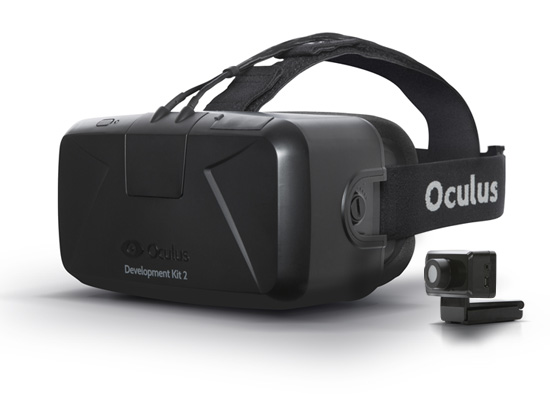
\includegraphics[width=0.6\textwidth]{Figs/oculus.jpg}
\caption{The \textit{Oculus Rift DK2} Head-Mounted Display and position tracking camera \cite{Parisi15}.}
\label{fig:oculus}
\end{figure}
\textit{DK2} was released in 2014 as the successor of \textit{DK1}, with better resolution (1920 x 1080 pixels, 960 x 1080 per eye) and positional tracker, which was not introduced in a previous model. Therefore, it enables the user not only to look around, but also to move around a virtual scene.  For the head tracking purposes, \textit{Rift} combines inertial and magnetic tracking in so-called Inertial Measurement Unit (IMU) what results in a 3 DOF effect. 6 degrees of freedom are introduced by optical tracking, with usage of micro-LED markers on the headset and IR camera. Although this solution improves immersion effect, it is still not perfect, as the user needs to be in front of the tracking camera, what limits his area of movement. This issue is  going to be solved soon with introducing third generation of \textit{Oculus}, called \textit{Crescent Bay}, which has 360-degree head tracking and higher resolution of an image. 

What is more, \textit{Oculus} producer provides needed software, \textit{Oculus Runtime} and \textit{Software Development Kit} (SDK) for developers sake \cite{Parisi15, Oculus16}. Additional facilitation constitutes availability of engines that are strongly focused on developing applications for \textit{Rift}, like Unity3D.
\subsection{\textit{Google Cardboard}}
Introduced in 2014, \textit{Cardboard VR} hastens Virtual Reality experience possibility for an average consumer. Since it makes use of almost every smart phone (which are owned by a large part of society nowadays), it allows to immerse into VE without expensive hardware- neither HMD nor computer. \textit{Google Cardboard} is simply a box with two lenses, which should be set by a  user (Figure \ref{fig:cardboard}). 
\begin{figure}[h] 
\centering    
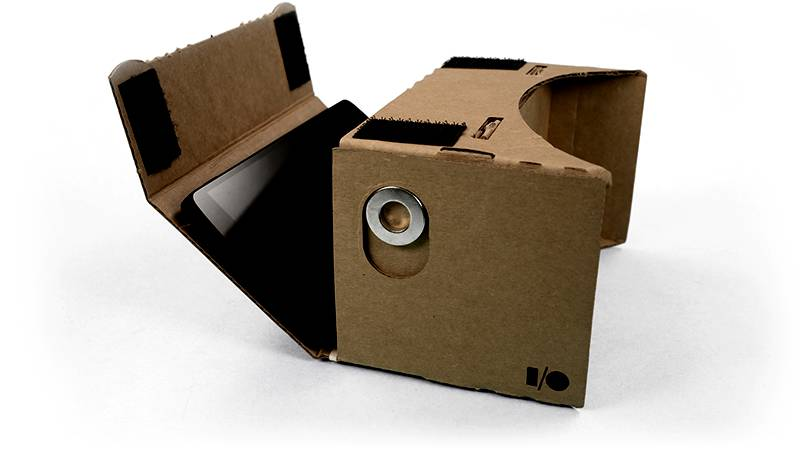
\includegraphics[width=0.6\textwidth]{Figs/cardboard.jpg}
\caption{The \textit{Google Carboard} VR viewer \cite{Parisi15}.}
\label{fig:cardboard}
\end{figure}
The stereoscopic image is created through the Cardboard-ready application on the phone, which should be placed inside the device. It provides 90° FOV and head tracking, which is generated by the phone's accelerometer and compass. Obviously, impression of immersion in this case is much smaller than in previously described device, but availability of this solution makes it more and more popular. In number of applications as well- hundreds of them are already accessible.

Similarly to \textit{Oculus Rift}, software for developers is also provided in this case by a producer. It exists in two options- an Android SDK and an add-in to, already mentioned, Unity3D engine \cite{Parisi15}.

\subsection{\textit{Leap Motion}}
\label{leapmotion}

Although it is not a Head-Mounted Display, like the previous examples, \textit{Leap Motion} provides user's input tool which is suitable for VR purposes. As this example of sensor device plays the key role in this work, it is described here as the only one of its kind.

Presented controller is a small peripheral USB device that uses two CCD IR cameras and three LED emitters, which generate IR light.  It tracks the position of predefined objects like palm and its finger tips in Cartesian space, relatively to to the center point of the device, which is placed at the position of the central IR emitter \cite{Weichert13}. Due to the difference in positions in which the controller may be used, it is worth mentioning that it employs right-handed Cartesian coordinate system, which is shown in Figure \ref{fig:leapCoordinates}.

\begin{figure}[h] 
\centering    
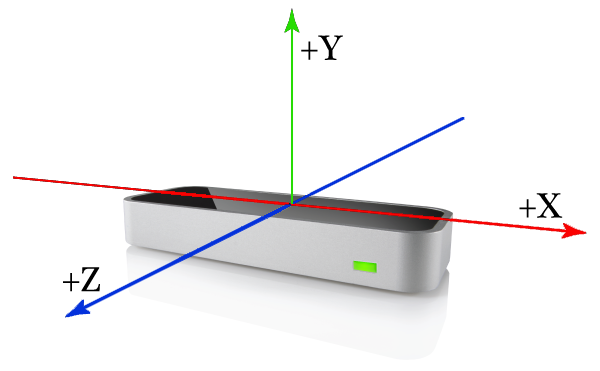
\includegraphics[width=0.6\textwidth]{Figs/leapCoordinates.png}
\caption{\textit{Leap Motion} controller and its coordinate system \cite{Leap16}.}
\label{fig:leapCoordinates}
\end{figure}

 According to the manufacturer data, the accuracy of the sensor in detection of fingertip position is approximately 0.01 mm, and the cameras frame rate varies from 20 to 200 fps depending on the user's settings and available computing power. \textit{Leap Motion} may be placed on a physical desktop or mounted onto Virtual Reality HMD. Its field of view is stated as 150° with a volume of approximately 0.23 cubic meters and the effective range varies between 25 and 600 mm above or before the device. 

 
\begin{figure}[h] 
\centering    
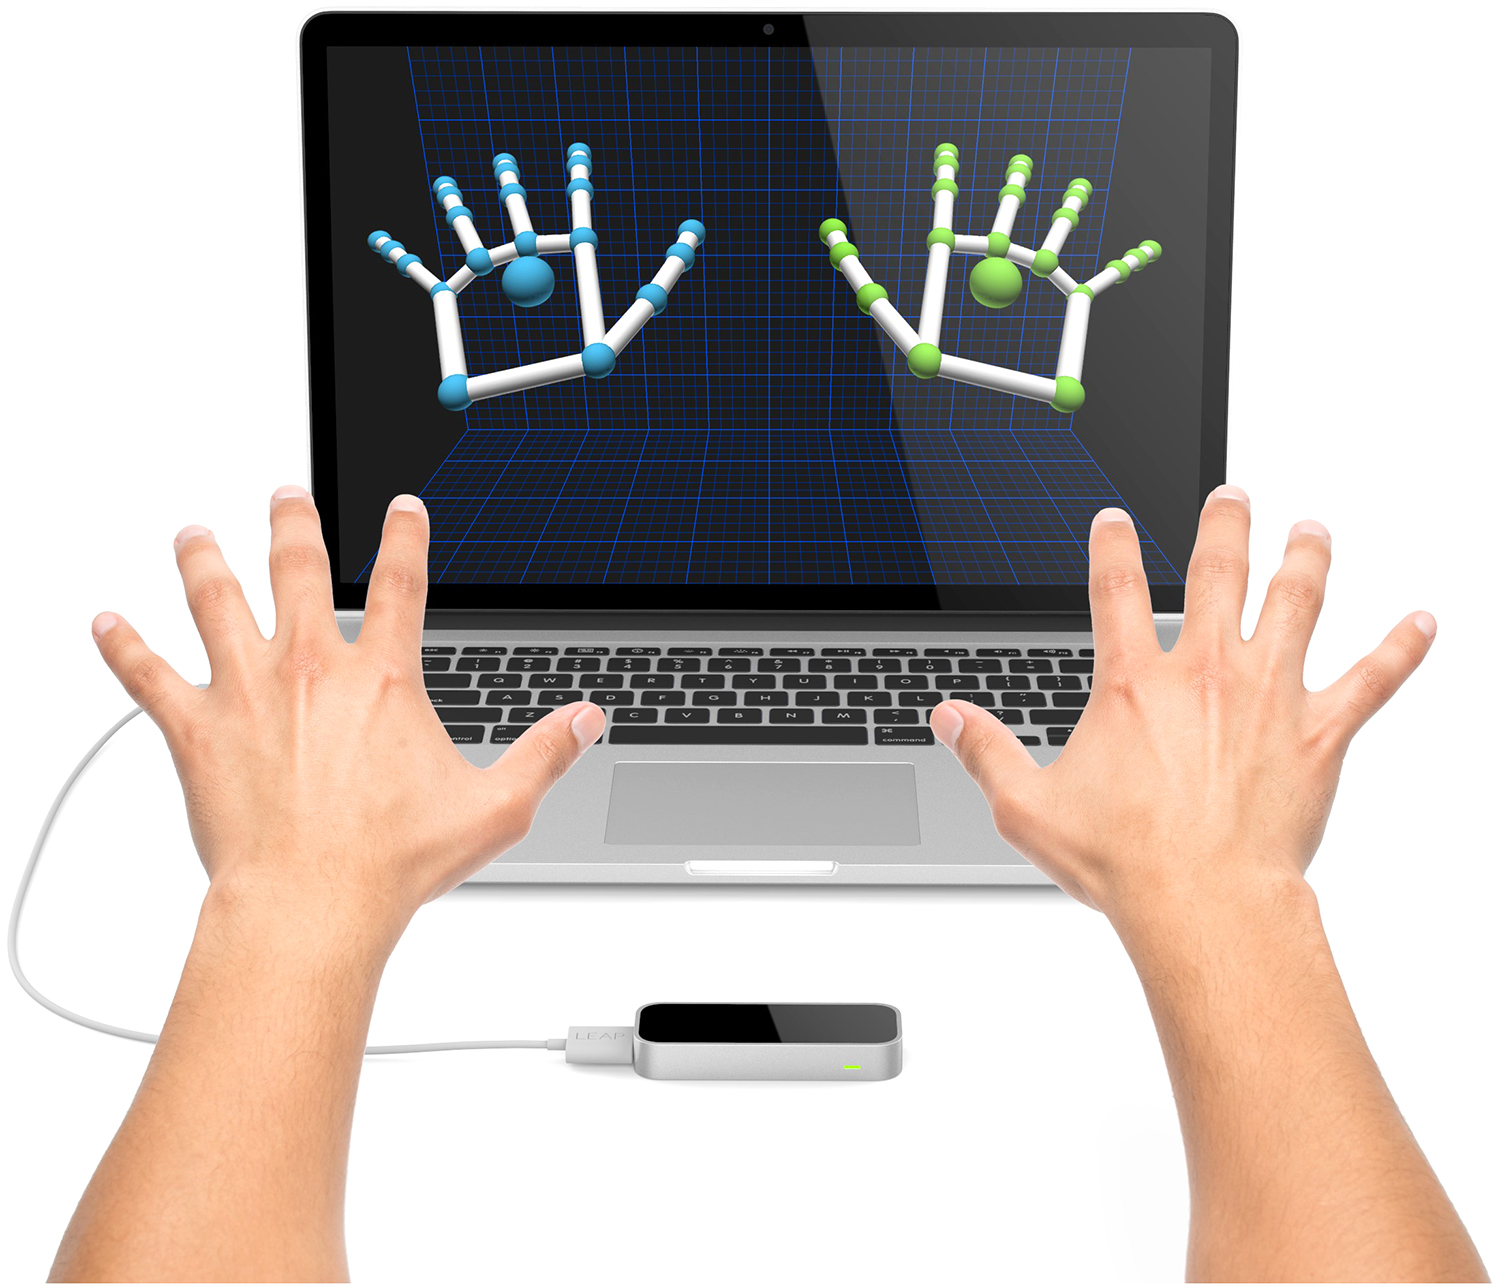
\includegraphics[width=0.4\textwidth]{Figs/leapmotion.jpg}
\caption{\textit{Leap Motion} in use- hand models on the screen are corresponding with the tracked real hands of the user \cite{Leap16}.}
\label{fig:leapmotion}
\end{figure}

The \textit{Leap Motion} API (Application Programming Interface) measures distance, time, speed and angle of the objects recorded by cameras. The software uses an internal model of human hand, what enables predictive tracking in case of temporary visibility disturbances. Moreover, the model contains all anatomical finger bones. Thanks to that, visualisation of hands in the three-dimensional VR scene is more immersive, as the model's movements are very close to its real equivalent (Figure \ref{fig:leapmotion}).
The most recent hand tracking software release, called \textit{Orion} indicates variety of improvements, dedicated mostly for VR purposes. Additionally, for the developer's use, \textit{Leap Motion} offers its SDK with libraries needed for the application development. It is available in several languages and enables integration with Unity3D engine.

%********************************** % Fifth Section  *************************************
\section{Possible applications}%Section - 1.5 
There is a large variety of applications in which Virtual Reality is and may be involved. List of possibilities constantly grows with the VE development, where entertainment constitutes the group of one of the strongest commercial potential. Therefore, many developer tools are mainly focused on creating video games, which may become more and more involving thanks to or because of VR. What is more, it creates a new way of thinking about social media and web browsing. The same happens to live entertainment- some of the famous artists have already broadcast their shows in the VE versions, making attending it possible to larger group of fans. 

But not only amusement makes Virtual Environment such an interesting and unique platform. Another industry is widely understood education. By providing interactive learning, VR may contribute to the increase of effectiveness in educating process. Thus simulations, such as medical training scenarios, scientific laboratory, flight or military reproductions, which are already created and developed, may become indispensable part of different training processes, preparing for the most unusual cases in a safe and inexpensive way. Moreover, simulations that simply create 3D VR representations may also be a valuable tool, immersing the user and facilitating understanding of presented image. That issue may be used in scientific sector, what is strongly connected with the topic of this work and described later in Chapter \ref{chapter2}. What is more, medical applications of VR are not only connected with the personnel's education. Creating the virtual world provides a platform for a new type of therapies, especially psychotherapies (like anxiety treatment) or even diagnosis, comparing reactions of possible patient with a healthy group. This topic is of great interest in a scientific world nowadays, resulting in a number of publications describing new treatment ideas.

Another field where VR is already applied is an architecture together with real estate. Creating visualisations in three dimensional view is not only a feature for designers purposes, but most of all to customers. They may experience their presence in presented properties quickly and easy, both by watching projects or video presenting already existing places. This function is also used in tourism, where showing hotel room or aeroplane interior in VR may be important for the sale success. Additionally, for those who cannot travel, VE may offer tours without getting out from their home. \cite{Parisi15, Singal15}


Examples presented here are just a few of the many other possibilities, that are constantly created. In all of them Virtual Reality facilitates or even enables humans life, and with the growing availability of VE gear it soon may become part of their every-day reality.

%makeindex <filename>.nlo -s nomencl.ist -o <filename>.nls
\nomenclature[z-API]{API}{Application Programming Interface}
\nomenclature[z-AR]{AR}{Augmented Reality}
\nomenclature[z-AV]{AV}{Augmented Virtuality}
\nomenclature[z-CPU]{CPU}{Central Processing Unit}
\nomenclature[z-DOF]{DOF}{Degree of Freedom}
\nomenclature[z-EOG]{EOG}{Electro-Oculography}
\nomenclature[z-FOV]{FOV}{Field of View}
\nomenclature[z-GPU]{GPU}{Graphics Processing Unit}
\nomenclature[z-HMD]{HMD}{Head-Mounted Display}
\nomenclature[z-IDE]{IDE}{Integrated Development Environment}
\nomenclature[z-IMU]{IMU}{Inertial Measurement Unit}
\nomenclature[z-IR]{IR}{Infrared}
\nomenclature[z-LOD]{LOD}{Level of Detail}
\nomenclature[z-MR]{MR}{Mixed Reality}
\nomenclature[z-RE]{RE}{Real Environment}
\nomenclature[z-SDK]{SDK}{Software Development Kit}
\nomenclature[z-VE]{VE}{Virtual Environment}
\nomenclature[z-VR]{VR}{Virtual Reality}
\nomenclature[z-WOW]{WOW}{Window on World}

